in der messung in davos \ref{} wurde der vergleichbare unveränderte schnee wiederholt gemessen. 

\begin{figure}
    \centering
    \includegraphics[width=0.8\textwidth]{Bilder/Varianz.png}
    \caption{10 Messungen von vergleichbarem unverändrtem Schnee}
    \label{fig:Varianz}
\end{figure}


In dem Bild \ref{img:Varianz} wurde Schnee in einer $0,2 m^2$ Fläche gemessen. Ziel war es, die Varianz von vergleichbarem Schnee zu ermitteln. Die Varianz zwischen den einzenlen Tapes ist hoch.


Mit Ishikawa \ref{fig:IshikwaDavos} wurde das Problem der hohen Varianz genauer analysiert.



\begin{figure}
    \centering
    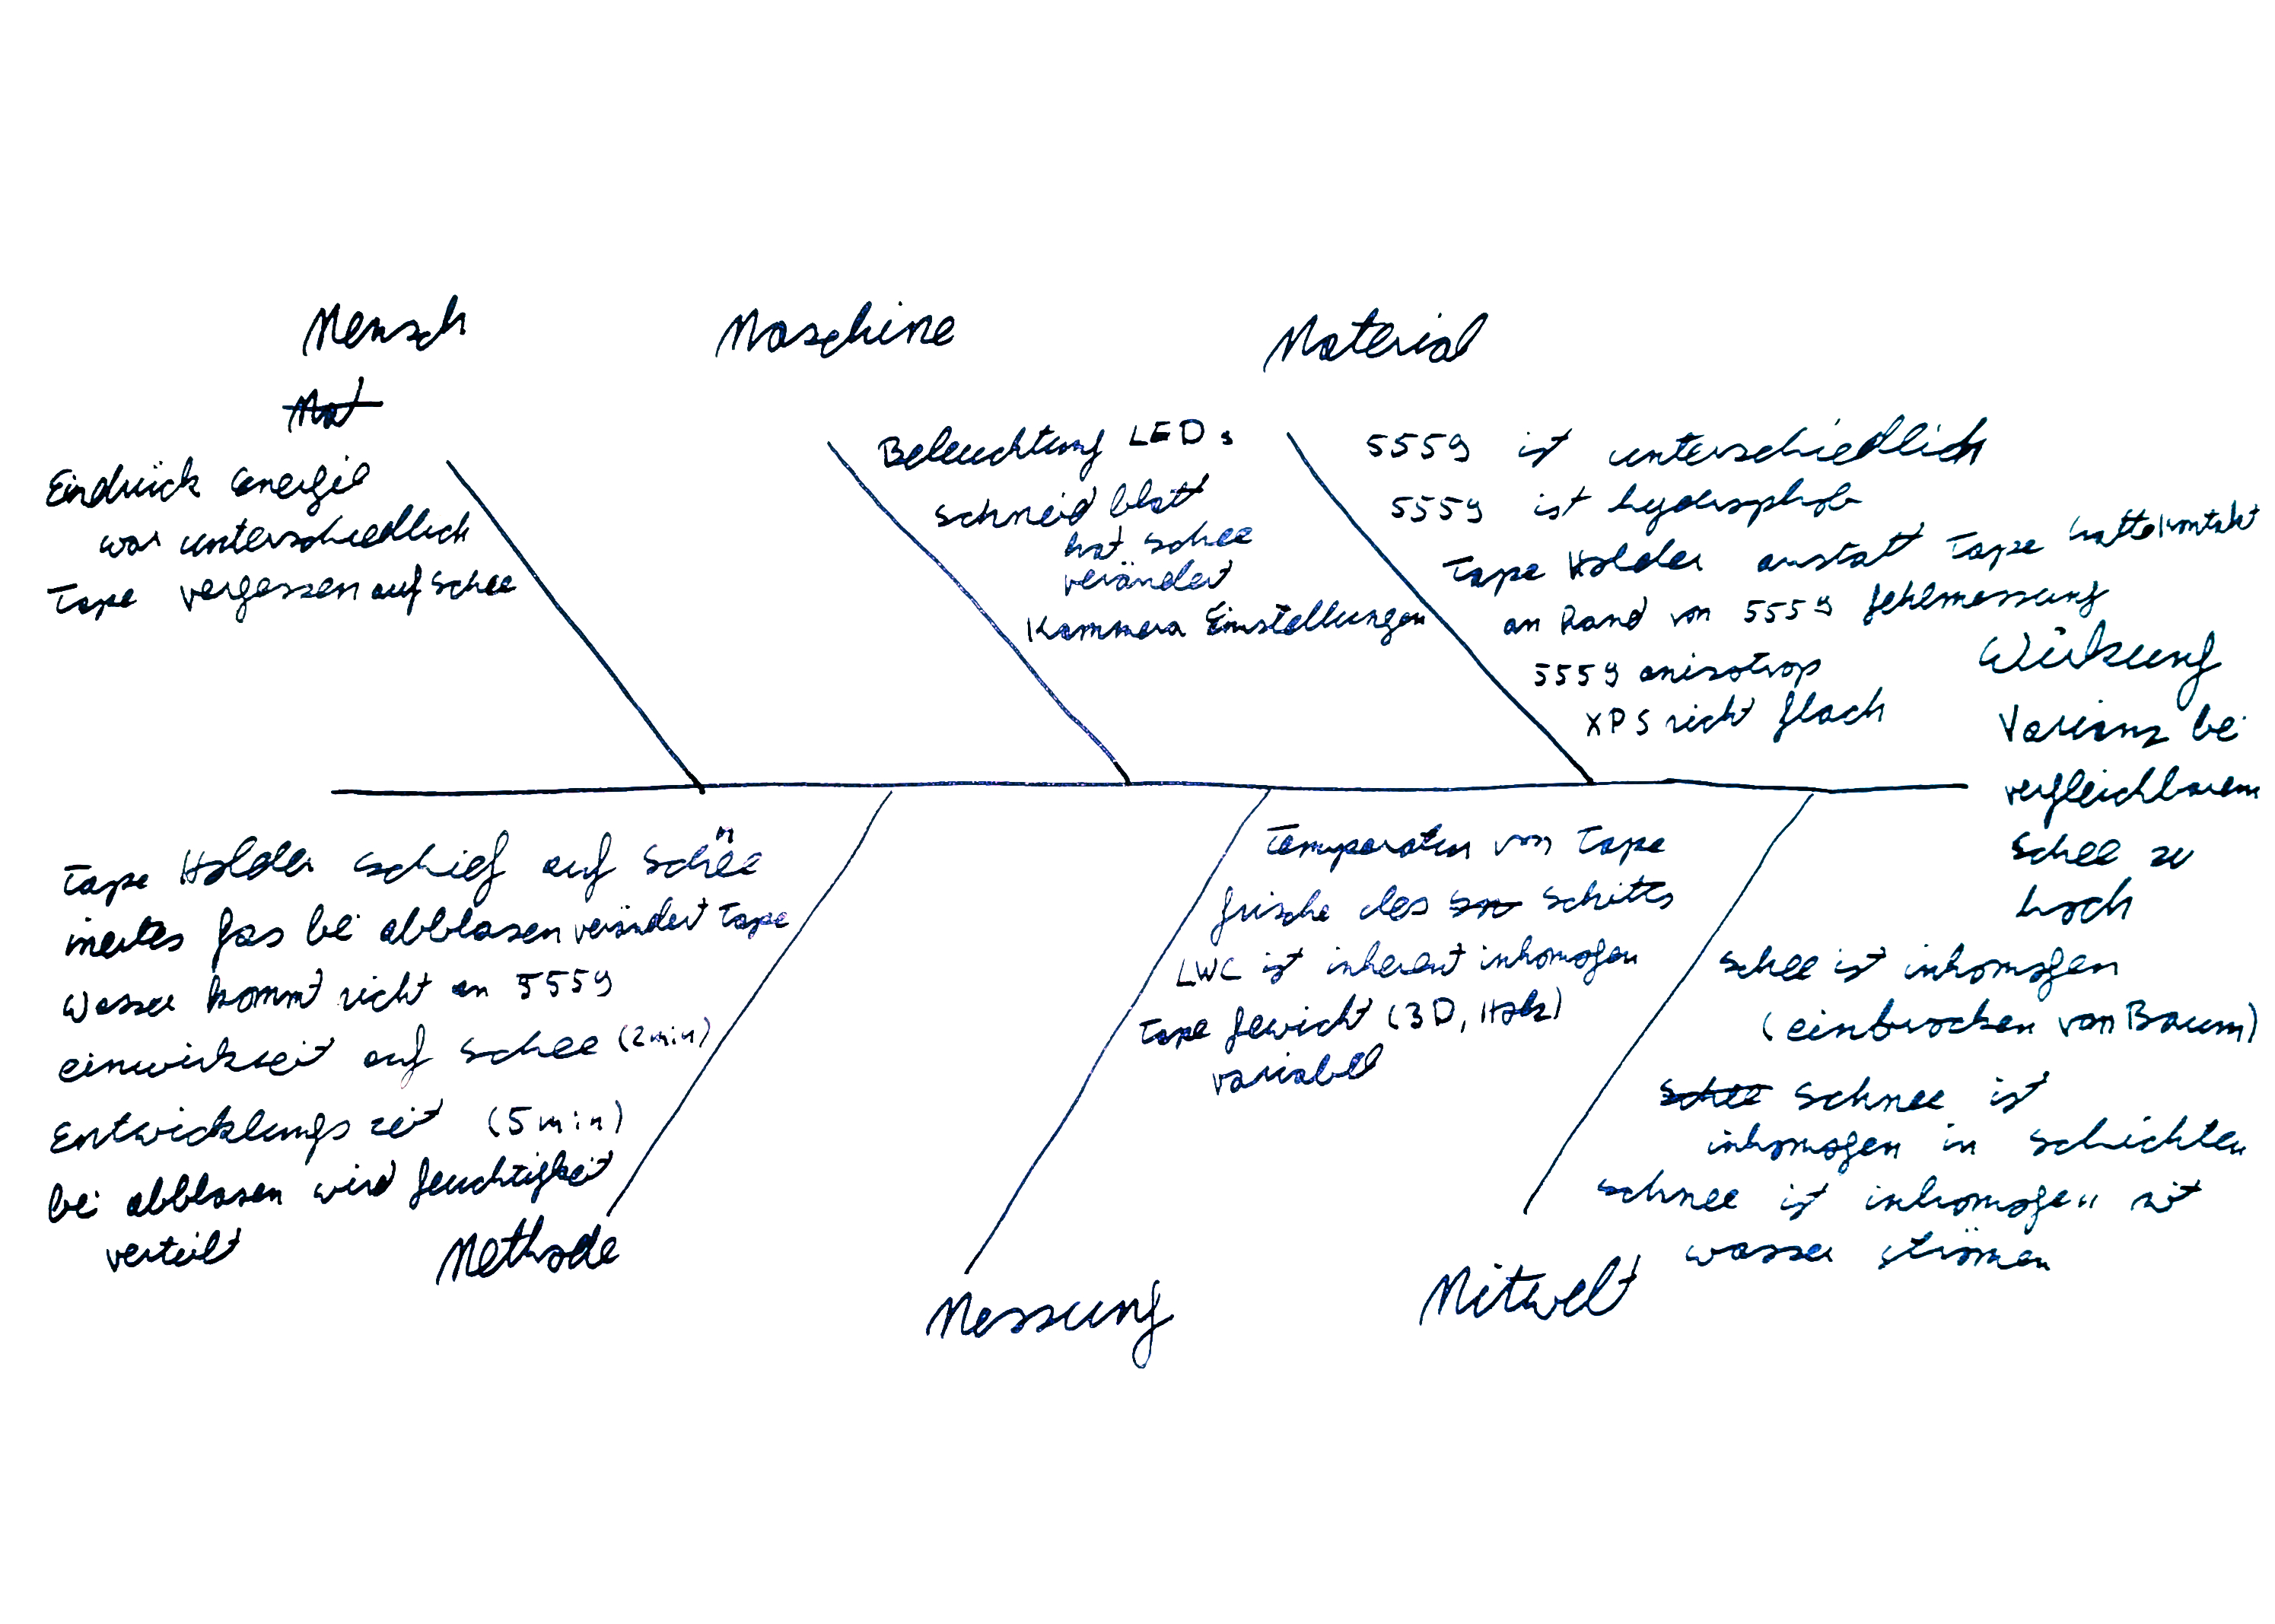
\includegraphics[width=0.8\textwidth]{Bilder/IshikawaDavos.jpg}
    \caption{Ishikawa Fehler Analyse für die Messung des Funktionsmusters 2}
    \label{fig:IshikwaDavos}
\end{figure}




Die wichtigsten Einflüsse sind:
\begin{itemize}
\item Das Tape ist anisotrop durch die Herstellung. Das ist besonders auffällig an den Rändern. Die Lösung wurde in \ref{fig:Bildverarbeitnugskonzpet} schon intuitiv benutzt. Der Rand (etwa 2 mm) soll nicht beachtet werden. Der Bildausschnitt wird in Zukunft so gewählt, dass der Rand nicht im Bild ist.
\item Das Tape hat einen schlechten Kontakt zum Wasser auf dem Schnee. Um diese Hypothese zu überprüfen, wurde der Winkel eines Wassertropfens auf dem Tape gemessen. Mit einem Winkel von 90 Grad ist das Tape genau zwischen hydrophob und hydrophil.
\item Die Beleuchtung war nicht homogen. Deswegen werden LEDs mit Diffusoren im nächsten \ref{} Funktionsmuster verbaut.
\item Die Tape-Halter standen nicht genau senkrecht. Deswegen wurde die Führung mit den Magnetbögen und Stativmaterial gebaut.
\item Die Eindrückenergie war inkonsistent. Deswegen wurden die Hauptzahl der Versuche ohne extra Energie durchgeführt. Bei dem Durchgang mit Energie wurde das Stativmaterial benutzt, um eine gleiche potentielle Energie sicherzustellen.
\item Der Tapehalter und nicht das Tape hatten Kontakt zum Schnee. Deswegen wurde der neue Tapehalter umkonstruiert, sodass 40 mm nur der XPS-Schaumstoff mit dem Tape in den Schnee eindringen kann.
\item Der XPS-Schaumstoff ist nicht flach. Deswegen wurde eine Schneidlehre gebaut, um den XPS senkrecht zu schneiden. Weitere Möglichkeiten wären, eine Glasplatte (Mikroskop-Objektträger) zwischen den XPS und das Tape zu machen oder einen plastisch verformbaren Träger für das Tape zu entwickeln.
\item Die Temperatur des Tapes war vor dem Schneekontakt die Umgebungstemperatur (viel). Deswegen wurde jedes Tape runtergekühlt und mit der Wärmebildkamera überprüft.
\item Die Gewichte der Tapehalter waren um rund 10 % unterschiedlich, denn es wurden verschiedene Versionen benutzt. Die neue hat nur eine einzige Version an Tapehaltern.
\item Der Schnee ist inhomogen. Die Messung war unter einem Baum, von dem Schnee und Eis heruntergefallen waren. Das hat dazu geführt, dass im Schnee zentimetergroße Einregionen waren.
\item Der Schnee ist inhomogen in Schichten. In den nächsten Messungen wurde ein weniger geschichteter Schnee gewählt.
\item Der Schnee ist inhomogen mit Wasserströmen. Die Messung in Davos war in der Nähe eines Baches. Die nächste Messung wurde ein homogener Schnee gewählt.
\item Die Ebene, auf der das Tape geklebt ist, ist nicht eben, sondern beim Transport eingedrückt worden. Um das Problem zu reduzieren, wurden Pelican Boxen für den Transport benutzt.
\end{itemize}

Weitere mögliche Gründe und die Strukturierung der Gründe können im Ishikawa-Diagramm gesehen werden \ref{fig:IshikwaDavos}.



\begin{figure}
    \centering
    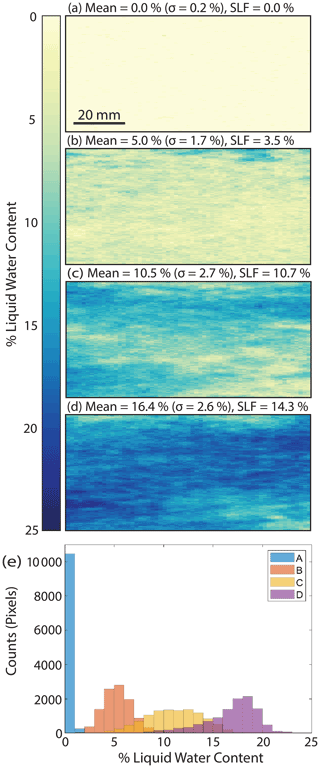
\includegraphics[width=0.8\textwidth]{Bilder/tc-16-43-2022-f08-thumb.png}
    \caption{Ishikawa Fehler Analyse für die Messung des Funktionsmusters 2}
    \label{fig:IshikwaDavos}
\end{figure}

